%%%%%%%%%%%%%%%%%%%%%%%%%%%%%%%%%%%%%%%%%
% Journal Article
% LaTeX Template
% Version 1.3 (9/9/13)
%
% This template has been downloaded from:
% http://www.LaTeXTemplates.com
%
% Original author:
% Frits Wenneker (http://www.howtotex.com)
%
% License:
% CC BY-NC-SA 3.0 (http://creativecommons.org/licenses/by-nc-sa/3.0/)
%
%%%%%%%%%%%%%%%%%%%%%%%%%%%%%%%%%%%%%%%%%

%----------------------------------------------------------------------------------------
% PACKAGES AND OTHER DOCUMENT CONFIGURATIONS
%----------------------------------------------------------------------------------------

\documentclass[oneside, 11pt, a4paper]{article}
\usepackage{polski}
\usepackage[utf8]{inputenc} 
\usepackage{cite}

\usepackage{graphicx}

\usepackage{lipsum} % Package to generate dummy text throughout this template

\usepackage[sc]{mathpazo} % Use the Palatino font
\usepackage[T1]{fontenc} % Use 8-bit encoding that has 256 glyphs
\linespread{1.05} % Line spacing - Palatino needs more space between lines
\usepackage{microtype} % Slightly tweak font spacing for aesthetics

%\usepackage[hmarginratio=1:1,top=32mm,columnsep=20pt]{geometry} % Document margins
\usepackage[top=3cm, bottom=3cm, left=2.5cm, right=2.5cm, columnsep=8mm]{geometry}

\usepackage{multicol} % Used for the two-column layout of the document
\usepackage[hang, small,labelfont=bf,up,textfont=it,up]{caption} % Custom captions under/above floats in tables or figures
\usepackage{booktabs} % Horizontal rules in tables
\usepackage{float} % Required for tables and figures in the multi-column environment - they need to be placed in specific locations with the [H] (e.g. \begin{table}[H])
\usepackage{hyperref} % For hyperlinks in the PDF

%\usepackage{lettrine} % The lettrine is the first enlarged letter at the beginning of the text


\usepackage{paralist} % Used for the compactitem environment which makes bullet points with less space between them

\usepackage{abstract} % Allows abstract customization
\renewcommand{\abstractnamefont}{\normalfont\bfseries} % Set the "Abstract" text to bold
\renewcommand{\abstracttextfont}{\normalfont\itshape} % Set the abstract itself to small italic text

\renewenvironment{abstract}
               {\list{}{}%
                \item[\textbf{Streszczenie.}]\relax}
               {\endlist}



\usepackage{titlesec} % Allows customization of titles
\usepackage[labelsep=period,font=small,format=plain,labelfont=bf,textfont=up]{caption}

% \DeclareCaptionFormat{myformat}{\fontsize{10}{11}\selectfont#1#2#3}
% \captionsetup{format=myformat}

\DeclareUnicodeCharacter{00A0}{ } % solution for "Unicode char \u8:  not set up for use with LaTeX."

%\renewcommand\thesection{\Roman{section}} % Roman numerals for the sections
%\renewcommand\thesubsection{\Roman{subsection}} % Roman numerals for subsections
\titleformat{\section}[runin]{\bfseries\centering}{\thesection.}{3pt}{} % Change the look of the section titles
%\titleformat{\subsection}[]{}{}{}{}[]
\titleformat{\subsection}[runin]{\bfseries}{\thesubsection.}{3pt}{} % Change the look of the section titles
\titlespacing*{\section}{0pt}{6pt}{3pt}[0pt]
\titlespacing*{\subsection}{0pt}{3pt}{3pt}[0pt]

\usepackage{fancyhdr} % Headers and footers
\pagestyle{fancy} % All pages have headers and footers
\fancyhead{} % Blank out the default header
\fancyfoot{} % Blank out the default footer
\renewcommand{\headrulewidth}{0pt}

%\fancyhead{} % Custom header text
\fancyfoot[RO,LE]{\begin{center}\thepage\end{center}} % Custom footer text

\renewcommand{\abstractname}{Streszczenie.}    % clear the title
\renewcommand{\absnamepos}{empty} % originally center
\setlength{\parindent}{0.4cm}

 \setlength{\parskip}{0mm}
 \let\oldbibliography\thebibliography
\renewcommand{\thebibliography}[1]{\oldbibliography{#1}
\setlength{\itemsep}{0pt}} %Reducing spacing in the bibliography.


%----------------------------------------------------------------------------------------
% TITLE SECTION
%----------------------------------------------------------------------------------------

\title{\vspace{15mm}\fontsize{14pt}{10pt}\selectfont\textbf{Problematyka rozproszonych systemów - przypadek \emph{Apache Cassandra}}} % Article title

\author{
{\fontsize{12pt}{1.2em}\selectfont Marek Lewandowski} \\
{\fontsize{11pt}{1.2em}\selectfont Wydział Elektroniki i Technik Informacyjnych, Politechnika Warszawska} \\
{\fontsize{11pt}{1.2em}\selectfont \href{mailto:marek.m.lewandowski@gmail.com}{marek.m.lewandowski@gmail.com}} 
\date{}
}


%----------------------------------------------------------------------------------------

\begin{document}

\maketitle % Insert title

\thispagestyle{fancy} % All pages have headers and footers

%----------------------------------------------------------------------------------------
% ABSTRACT
%----------------------------------------------------------------------------------------



%----------------------------------------------------------------------------------------
% ARTICLE CONTENTS
%----------------------------------------------------------------------------------------

\begin{multicols}{2} % Two-column layout throughout the main article text

%\begin{abstract}
\section*{Streszczenie.}

\textit{
Artykuł omawia nierelacyjne bazy danych i twierdzenia z nimi związane takie jak \emph{CAP, BASE}. W szczególności omawia cechy szczególne i budowę bazy \emph{Apache Cassandra}. \emph{Apache Cassandra} jest kanoniczną nierelacyjną bazą danych, której zrozumienie znacząco ułatwia zrozumienie większości pozostałych nierelacyjnych baz danych.
}

\section{Motywacja.}
Nierelacyjne bazy danych powstały, w celu rozwiązania nowego rodzaju problemów, którym nie były w stanie sprostać tradycyjne bazy danych. Problemy to bardzo duża, szybko przyrastająca ilość danych oraz potrzeba obsługi równie dużego obciążenia systemu.

Ilość danych, wyrażana może być, aż peta bajtach ($1PB=1000 TB$), co może sprawiać problemy jeśli chcielibyśmy obsłużyć taką ilość danych jednym komputerem. W związku z tym poruszamy się po dziedzinie klastrów serwerów, a nie pojedynczych maszyn. Pojedyncza maszyna to również pojedynczy punkt awarii. Takie i inne problemy adresowane są przez nierelacyjne bazy danych.

Często podczas omawiania nierelacyjnych baz danych przytacza się przypadek firmy \emph{Amazon}. \emph{Amazon} oświadczył, że wzrost czasu odpowiedzi w ich serwisie o 0.1 sekundy powoduje spadek sprzedaży o 1\%. Wysoka wydajność i niski czas dostępu są możliwe dzięki nierelacyjnym bazom danych oraz innym pobocznym technikom. Warto zatem pamiętać o biznesowej wartości tych rozwiązań, wiedzieć jak działają i jakim prawom podlegają.

\section{Spójność i dostępność}
W klasycznych bazach danych, często słyszymy o tym, że baza jest spójna. Taka spójność oznacza, że wszystkie mechanizmy w bazie takie jak więzy integralności, klucze obce, ograniczenia na kolumny są spełnione. Chcę przedstawić inną definicję spójności.

Spójność oznacza jedną wersję danych, a więc wszystkie takie same dane, są zawsze w identycznej wersji. Dostępność rozumiana jest jako zdolność systemu do obsługi żądania zapisu/odczytu danych i zwrócenia odpowiedzi. 

\emph{ACID} charakteryzuje klasyczne bazy danych, które posiadają bardzo wysoką spójność. \emph{BASE} to akronim, który należy omówić. 

\begin{compactitem}
  \item większość danych dostępna przez cały czas (ang. Basically Available)
  \item dane wystarczająco świeże (ang. Soft state)
  \item osiągnięcie spójności odsunięte w czasie, ale osiągalne (ang. Eventually consistent)
\end{compactitem}

\emph{ACID} i \emph{BASE} reprezentują dwa podejścia projektowe po przeciwnych końcach spektrum spójność\dywiz dostępność. Naturalnie \emph{ACID} znajduje się po stronie spójności i reprezentuje klasyczne podejście do baz danych. \emph{BASE} znajduje się po przeciwnej stronie spektrum i reprezentuje systemy z dużą dostępnością. Dzięki tym modelom wybór pomiędzy dostępnością, a spójnością jest jawny.


\section{Twierdzenie CAP.}
Brewer opublikował w 1999 roku \cite{Fox99harvest} twierdzenie przedstawiające wybór dwóch z trzech cech w rozproszonych bazach danych. Dwie cechy już znamy. Należy wytłumaczyć czym jest odporność na partycje. 

Partycja w rozprosznym systemie występuje, wtedy gdy część węzłów w klastrze nie ma łączności z co najmniej jednym węzłem, inaczej mówiąc klaster jest podzielony na dwie części, które nie mogą się ze sobą komunikować. Taka sytuacja może wystąpić w co najmniej dwóch przypadkach. Część maszyn może ulec awarii i tym samym zniknie z klastra na długi czas, a więc będzie niedostępna z punktu widzenia pozostałych maszyn. Inną możliwością jest brak łączności spowodowany awarią sieci. Z punktu widzenia maszyn w klastrze obie sytuacje są identyczne i nie da się ich rozróżnić. W obu tych sytuacjach występuje partycja rozdzielająca maszyny na dwie grupy.
 Twierdzenie Brewera mówi, że można mieć jedynie dwie cechy z poniższych:
\begin{compactitem}
  \item spójność,
  \item dostępność,
  \item odporność na partycje.
\end{compactitem}

W przypadku rozproszonych systemów brak odporności na partycje to pojedyczny punkt awarii. Wystarczy sobie wyobrazić, że pojedyncza maszyna ulega awarii, a baza nie jest w stanie dalej funkcjonować. Z tego powodu rozważa się wybór pomiędzy dostępnością, a spójnością. Odporność na partycje powinna być zawsze. Można zatem mówić o binarnym wyborze.

Binarny wybór został zaprezentowany w oryginalnej postaci twierdzenia. Przez ponad dekadę powstało wiele typów systemów, które skupiają się na innych kombinacjach właściwości. 
\subsection{Twierdzenie dzisiaj.} Wokół twierdzenia pojawiło się wiele nieporozumień. Przez lata odkryto sporo niuansów. Właściwości nie są binarne, a bliżej im do wartości ciągłych. Dostępność jest w zakresie procentowym. Istnieje wiele poziomów spójności. Węzły w klastrze mogą nie zgadzać się co do tego czy partycja faktycznie występuje. Autor opublikował 12 lat później artykuł \cite{Brewer:2012ba}, który rozwiewa większość wątpliwości.

Dzisiaj możemy przedstawić twierdzenie w lepszy sposób. Podczas wystąpienia partycji niemożliwa jest idealna spójność i idealna dostępność. Dzięki specjalnej obsłudze systemu podczas partycji, można mieć więcej niż tylko jedną cechę. Wymaga to użycia odpowiednik technik. Jedną z technik jest ograniczenie możliwych operacji, tylko do tych, które nie zniszczą spójności. Przykładem rozprosznego systemu, który stosuje taką technikę jest \emph{Google Docs}, który podczas braku połączenia (partycji), udostępnia tylko część narzędzi tesktowych. 

Jeśli partycja nie występuje system może mieć idealną dostępność i spójność. Dopiero podczas wystąpienia partycji należy dokonać wyboru pomiędzy spójnością, a dostępnością lub mieć specjalny tryb operacji podczas partycji. Nie dokonanie wyboru w krótkim czasie to wybór spójności, ponieważ żądanie nie zostanie obsłużone w odpowiednim czasie, a więc z perspektywy klienta system nie będzie dostępny.

\section{Parametry nierelacyjnych baz danych.}
Nierelacyjne bazy danych często posiadają trójkę parametrów, których manipulacja pozwala osiągnąć różne tryby pracy systemu. Repliką nazywamy węzeł odpowiedzialny za przechowywanie tych samych danych.

\begin{compactitem}
  \item \textbf{$N$} - liczba replik, do których zapisuje się dane,
  \item \textbf{$W$} - liczba potwierdzeń zapisu potrzebna do poprawnego zapisu,
  \item \textbf{$R$} - liczba replik, z których się czyta.
\end{compactitem}

Tabela \ref{tab:parametry} pokazuje przypadki charakterystyczne ustawień parametrów. Jak widać, może uzyskać bardzo różne zachowanie bazy danych w zależności od wartości powyższych parametrów.

\begin{table}[H]
\centering

\begin{tabular}{|c|c|l|}
\hline
\textbf{R} & \textbf{W} & \textbf{Charakterystyka}                                                         \\ \hline
1          & N          & \begin{tabular}[c]{@{}l@{}}Wysoka spójność, \\ bardzo szybki odczyt\end{tabular} \\ \hline
N          & 1          & \begin{tabular}[c]{@{}l@{}}Wysoka spójność, \\ bardzo szybki zapis\end{tabular}  \\ \hline
1          & 1          & \begin{tabular}[c]{@{}l@{}}Niska spójność, \\ bardzo szybki odczyt i zapis \end{tabular} \\ \hline
\end{tabular}
\captionsetup{justification=centering}
\caption{Przypadki charakterystyczne wartości parametrów N,R,W.}
\label{tab:parametry}
\end{table}

\vspace{-5mm}
\subsection{Reguła spójności.}
Istnieje reguła dotycząca parametrów, która jeśli spełniona gwarantuje zachowanie spójności. Jeśli nierówność $R + W \geq N + 1$ jest spełniona, to każdy odczyt otrzyma najnowszą wersję danych. Ze wzoru widać, że zapis i odczyt zazębia się na większości replik, dlatego też zawsze będą dostępne najświeższe wersje danych. 

Można zadać pytanie w jaki sposób reprezentowana jest świeżość danych. Istnieje kilka technik \cite{Lamport:1978jq} \cite{fidge1988timestamps}, które to umożliwają. Poznamy jedną z nich użytą w bazie \emph{Apache Cassandra}.

\section{Apache Cassandra.}
Nierelacyjna baza danych, zapewniająca wysoką dostępność i odporność na partycje. Cechuje ją liniowa skalowalność. Jeśli mając $6$ węzłów możemy obsłużyć $200 000$ żądań zapisu na sekundę to mając $12$ obsłużymy $400 000$ żądań. Architektura \emph{Cassandry} spełnia założenia \emph{Dynamo} \cite{DeCandia:2007:DAH:1323293.1294281}, a więc węzły są równorzędne i symetryczne. Dane są replikowane na wielu węzłach. Skaluje się horyzontalnie, poprzez dodawanie kolejnych węzłów w trybie pracy ciągłej. Wykorzystuje takie same techniki jak \emph{Dynamo} dla problemów takich jak przywrócenie węzła ze stanu awarii, wykrycie nowego węzła w klastrze, wykrycie awarii węzła w klastrze, obsługa tymczasowej awarii. \emph{Cassandra} od \emph{Dynamo} różni się modelem danych. \emph{Dynamo} posiada model danych, który w dużym uproszczeniu jest mapą klucz\dywiz wartość. \emph{Cassandra} posiada model danych oparty o \emph{Google BigTable} \cite{Chang:2006:BDS:1267308.1267323}, w którym to dane są przechowywane w kolumnach.

\subsection{Liniowa skalowalność.}
\emph{Cassandra} posiada liniową skalowalność dzięki mechanizmowi spójnego mieszania kluczy. \cite{Karger:1999kd}. Węzły tworzą pierścień. Pierścień mieści w sobie wszystkie wartości kluczy funkcji mieszającej. Węzły odpowiedzialne są za kolejne partycje kluczy. W przypadku pierścienia z 4 węzłami, pierścień podzielony jest na 4 partycje, gdzie każda partycja przypada na jeden węzeł. Sytuacja ta jest zilustrowana na rysunku \ref{fig:ring}. Wartości kluczy w zakresie od $-2^{63} $ do $2^{63} - 1$ rozłożone są na pierścieniu.

Aby odwołać się do danych w \emph{Cassandrze}, należy podać klucz partycjonujący. Z wartości tego klucza liczony jest skrót funkcją mieszająca. Typowo jest to funkcja mieszająca \emph{Murmur3}. Wynikiem jest wartość, która znajduje się na pierścieniu, a więc wiadomo, który węzeł odpowiada za te dane. Dostęp do danych ma zatem złożoność $\mathcal{O}(1)$.

Każdy węzeł jest równorzędny, można zatem pytać o dane dowolny węzeł, a ten przekieruje żądanie do odpowiedniego węzła.


 \begin{figure}[H]
 \centering
  \fbox{
    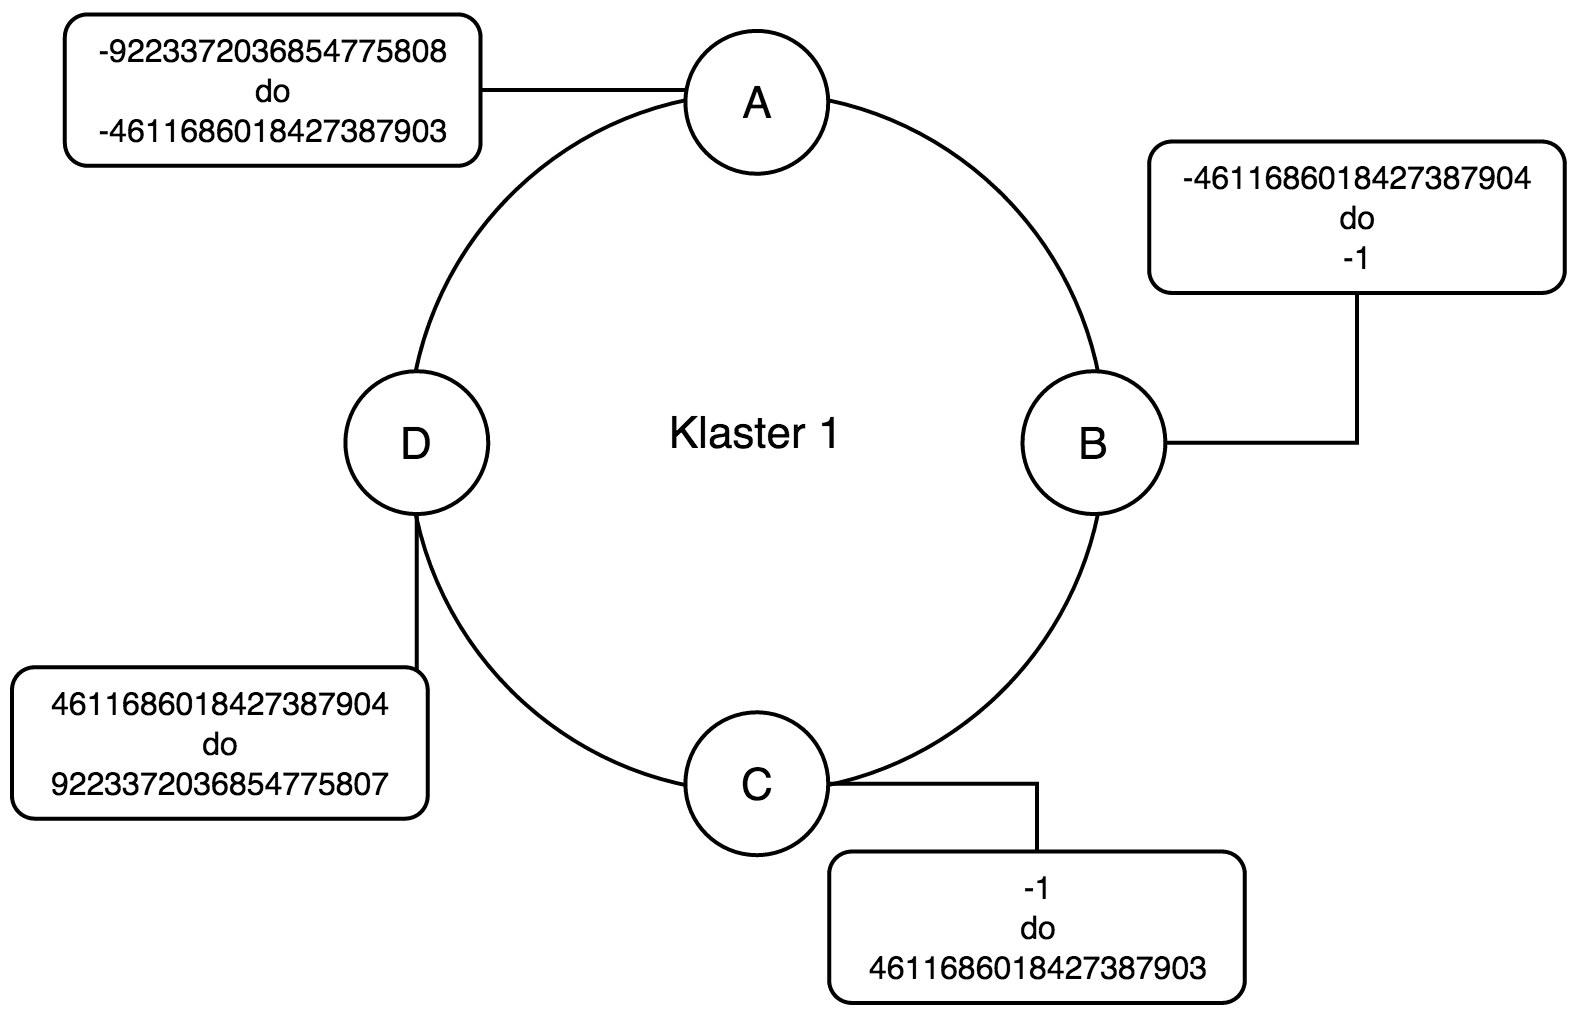
\includegraphics[scale=0.25]{./pierscien.png}
  }
  \begin{center}
  \captionsetup{justification=centering}
  \vspace{-3mm}
  \caption{Pierścień dla 4 węzłów}
  \label{fig:ring}
  \end{center}
  
\end{figure}
\vspace{-10mm}

\subsection{Replikacja danych}
W \emph{Apache Cassandra} dane są zorganizowane w tabelach, które w kolei należą do przestrzeni kluczy. Przestrzeń kluczy stanowi odpowiednik schematu bazy danych, w którym znajduja się tabele. Przestrzeni kluczy można mieć dowolnie dużo, podobnie jak tabel w każdej przestrzeni kluczy. Przy tworzeniu przestrzeni kluczy podaje się współczynnik replikacji $N$. Domyślną wartością jest $N=3$. 

Wracając do pierścienia z rysunku \ref{fig:ring}, dane z danej partycji replikowane są na kolejnych partycjach zgodnie ze wskazówkami zegara. Mianowicie, zakładając domyślny współczynnik replikacji, dane z węzła $A$ zreplikowane zostaną na węzłach $B$ i $C$. 

\subsection{Natywny model danych.}
\emph{Cassandra} posiada model danych oparty o \emph{BigTable}. W tym modelu danych dane są w kolumnach, które należą do wierszy, które należą do tabel. Nie istnieje żaden schemat danych, ponieważ każdy wiersz może mieć dowolne różne kolumny od innych wierszy. Kolumny w wierszach są posortowane po nazwach. 

Kolumna w \emph{Apache Cassandra} różni się jednak od zwykłej kolumny bazo\dywiz danowej. Kolumna, inaczej zwana komórką posiada:
\begin{compactitem}
  \item nazwę - kolumny są sortowane po nazwach
  \item wartość - miejsce na $2Gb$ danych
  \item znacznik czasowy - ostatnia data modyfikacji, bądź wstawienia komórki
  \item czas życia - opcjonalna wartość; wyrażona w sekundach, po upływie komórka zniknie z bazy danych
\end{compactitem}

Znacznik czasowy służy do określenia, która komórka jest najnowsza, a więc jest to mechanizm pozwalajacy na spójny odczyt danych. 

Każdy wiersz identyfikowany jest kluczem wiersza. Wynik funkcji skrótu od klucza wiersza określa pozycję na pierścieniu. Każdy wiersz może posiadać maksymalnie 2 miliardy komórek. Wiersz musi się fizycznie mieścić na jednym węźle. Choć każda komórka może posiadać maksymalnie $2Gb$ danych, w praktyce nie zaleca się przechowywania większej ilości danych niż kilka $Mb$ z racji tego, że dostęp do danych nie jest dostępem strumieniowym. Cała wartość jest odczytywana do pamięci i przekazywana dalej, a więc duże wartości mogą szybko wykorzystać pamięć, co doprowadzi do degradacji ogólnej wydajności węzła.

Czas życia jest bardzo przydatnym parametrem, ponieważ ma dużo praktycznych zastosowań. Pierwszym z brzegu jest ważność hasła. Jeśli hasło może być ważne 1 miesiąc, to można ustawić odpowiedni czas życia dla komórki przechowującej hasło. Jeśli przy odczycie nie będzie tej komórki to znaczy, że hasło wygasło. Podobny model można zastosować w wielu innych biznesowych sytuacjach.

\subsection{Model CQL.}
Model ten został stworzony jako dodatkowa warstwa abstrakcji nad natywnym modelem danych. \emph{Cassandra Query Language} pozwala na organizację danych w komórkach fizycznego wiersza, która przypominać będzie relacyjną bazę danych. Każdy fizyczny wiersz zawierać będzie wiele wierszy \emph{CQL}. Wiersze \emph{CQL} identyfikowane są poprzez klucz złożony z dwóch części. Cześć partycjonująca klucza jest dokładnie tym samym kluczem w przypadku modelu natywnego i identyfikuje wiersz w pierścieniu. Cześć sortująca identyfikuje wirtualny wiersz reprezentowany przez zestaw komórek w wierszu fizycznym. Cały mechanizm polega na odpowiednim nazewnictwie komórek. Klucz sortujący dołączony jest do nazwy każdej komórki fizycznej wraz z jej właściwą nazwą. Inaczej mówiąc, wartość klucza sortującego stanowi prefiks nazwy kolumny. Dzięki temu, że komórki posortowane są po nazwie, wiersz \emph{CQL} to zestaw kolejnych komórek o tym samym prefiksie.

W obecnej chwili model \emph{CQL} jest bardzo rozwijany i wszystko wskazuje na to, że \emph{CQL} będzie głównym medium modelowania danych. Należy jednak pamiętać o prawdziwej, natywnej reprezentacji danych.

Choć \emph{CQL} brzmi podobnie do \emph{SQL} należy pamiętać, że \emph{CQL} nie posiada większości funkcjonalności, którą oferują relacyjne bazy danych. Nie istnieją żadne złączenia, zagnieżdżone zapytania, sumowania oraz większość innych rzeczy. \emph{CQL} oferuje jedynie zapytanie typu \emph{SELECT ... FROM ... WHERE ...}. Każde zapytanie odczytu powinno dotyczyć jednego lub maksymalnie kilku wierszy. Inaczej tracona jest wydajność, ponieważ wymagane będzie zapytanie o dane kilka innych replik. Fizyczne wiersze rozsiane są na innych węzłach. Można się zatem zastanawiać w jaki sposób projektować systemy, które są banalne w małej skali w przypadku tradycyjnych baz danych.

\subsection{Modelowanie danych}
Poznaliśmy już modele danych. Warto powiedzieć w jaki sposób, można budować typowe aplikacje operate o \emph{Cassandrę}. Przy projektowaniu aplikacji wiemy w jaki sposób chcemy pytać o dane. Jeśli ktoś wybrał tą bazę to znaczy, że ma z tym problem. Przy modelowaniu tabel należy się zatem skupić na zapytaniach. Za przykład weźmy system, w których zbieramy dane o użytkownikach. Jednym z częstych zapytań jest zapytanie o użytkowników w danym mieście. Chcemy otrzymać listę użytkowników z danego miasta wraz z ich imieniem i nazwiskiem.

Bazę można traktować inaczej jako fabrykę indeksów. Dla użytkoników i wszystkich ich danych zbudowana zostanie jedna tabela. Dla powyższego zapytania zbudowana zostanie druga tabela, której kluczami wierszy będą nazwy miast. Przy dodawaniu użytkownika, będzie on również dodawany do drugiej tabeli pod odpowiednim miastem. Oprócz samego identyfikatora użytkownika pozwalającego na dostęp do jego wiersza skopiowane zostaną także imię i nazwisko. Tym sposobem odpowiedź na zapytanie przy takim modelu polega na odczycie jednego wiersza i wyświetleniu listy.

Podsumowując, modeluje się dane poprzez denormalizację i budowę wielu indeksów pokrywających wszystkie przypadki użycia danych, a więc w praktyce wszystkie zapytania odczytu.

\section{Przypadki użycia.}
\emph{Cassandra} idealnie nadaje się do przechowywania wszelkiego rodzaju danych ze znacznikami czasowymi, takimi jak logi, zdarzenia, pomiary. Poprzez użycie odpowiednik technik można sobie poradzić z obsługą bardzo dużej liczby żądań zapisu na sekundę. \emph{Cassandra} wykorzystywana jest do budowy silników rekomendacji, dynamicznych, wielowymiarowych rankingów. Przechowywane są w niej dane geograficzne.

\subsection{Przypadek \emph{I20 Water}} 
Firma ta wspiera różne firmy, które są dostawcami wody na świecie. Wspiera je poprzez inteligente rozwiązania monitorujące ciśnienie i wiele innych czynników w wodociągach, które odpowiednio zarządzają całą siecią wodociągową. Wodociąg posiada bardzo dużo fizycznych mierników, które mierzą te parametry i przesyłają je poprzez sieć \emph{GPS}, do głównego systemu. \emph{Cassandra} pozwala na zapis olbrzymiej ilości danych oraz szybki odczyt i analizę. Do analizy wykorzystywane są narzędzia, dobrze zintegrowane z \emph{Cassandrą}. Dzięki mierzeniu różnych parametrów i obserwację awarii sieci wodociągówej oraz szybką reakcję na takie sytuacje firma ta oszczędza 100 milionów litrów wody dziennie oraz obniżyła zużycie energii potrzebnej do pompowania wody o $20\%$.



%------------------------------------------------
%
%
%
%\section{Results}
%
%\begin{table}[H]
%\caption{Example table}
%\centering
%\begin{tabular}{llr}
%\toprule
%\multicolumn{2}{c}{Name} \\
%\cmidrule(r){1-2}
%First name & Last Name & Grade \\
%\midrule
%John & Doe & $7.5$ \\
%Richard & Miles & $2$ \\
%\bottomrule
%\end{tabular}
%\end{table}
%
%\lipsum[5] % Dummy text
%
%\begin{equation}
%\label{eq:emc}
%e = mc^2
%\end{equation}
%
%\lipsum[6] % Dummy text

%------------------------------------------------



%----------------------------------------------------------------------------------------
% REFERENCE LIST
%----------------------------------------------------------------------------------------

\bibliography{bibliography}{}
\bibliographystyle{plain}


%----------------------------------------------------------------------------------------

\end{multicols}

\end{document}